\newif\ifglobal

%%%%%%%%%%%%%%%%%%%%%%%
%%% Compile to view %%%
%%%%%%%%%%%%%%%%%%%%%%%

%%%%%%%%%%%%%%%%%%%%%%%%%%%%%%%%%%%%%%%%%%%%%%%%%%%
%%% Readme:                                     %%%
%%% https://www.overleaf.com/read/bwdjvfjksvjy/ %%%
%%%%%%%%%%%%%%%%%%%%%%%%%%%%%%%%%%%%%%%%%%%%%%%%%%%

% >>> M?: marks a module setting number or important notice

% >>> M4: Set {./relative-path} to external files for this module <<<
\def \modulefiles {./07-RESCLK}
% To add an external file, use:
% (Replace '---' with actual filename)
% '\input{\modulefiles/tables/---.tex}' for tables
% '\includegraphics{\modulefiles/figures/---}' for figures
% '\subfile{\modulefiles/---}' for register files


% >>> M1: This module is in global project? <<<
% 'YES' - uncomment; 'NO' - comment out
\globaltrue

\ifglobal
    \documentclass[main\_\_CN.tex]{subfiles}

\else
    % Font "FandolSong-Regular" used by ctex does not have GSUB table.
    % It causes warnings that do not affect compilation and can be ignored.
    \PassOptionsToPackage{quiet}{fontspec}

    \documentclass[openany, 10pt]{book}

    % >>> M2: In ./00-shared/preamble-trm-module, also find
    %         settings for visibility of todo notes, watermark <<<
    \usepackage{preamble-trm-module}


    % Enable Chinese typesetting
    \usepackage{ctex}

    % >>> M3: Temporary labels in Chinese
    %         you can add your own labels there <<<
    \myexternaldocument{./00-shared/temp-labels-cn}

\fi %\ifglobal


\setcounter{secnumdepth}{4}

% Define formatting of chapters in text
\setchineseformatting

% >>> M5: If this module needs any updates in
% './00-shared/preamble-trm-module.sty'
% (include additional package, etc.), contact your module PM
% or create the file './00-shared/changelog.tex' make the
% necessary updates yourself and document them in this file <<<

% Make text left-aligned and allow latex to break pages naturally, comment out for full justification
\raggedright
\raggedbottom


\begin{document}
\hypertarget{resclk}{}
\chapter{复位和时钟}
\label{mod:resclk}

\section{System 复位}
\subsection{概述}
系统提供三种级别的复位方式，分别是 CPU 复位，内核复位，系统复位。

所有的复位都不会影响 MEM 中的数据。
图 \ref{figure:Reset} 展示了整个子系统的结构以及每种复位方式：

\begin{figure}[H]
    \centering
    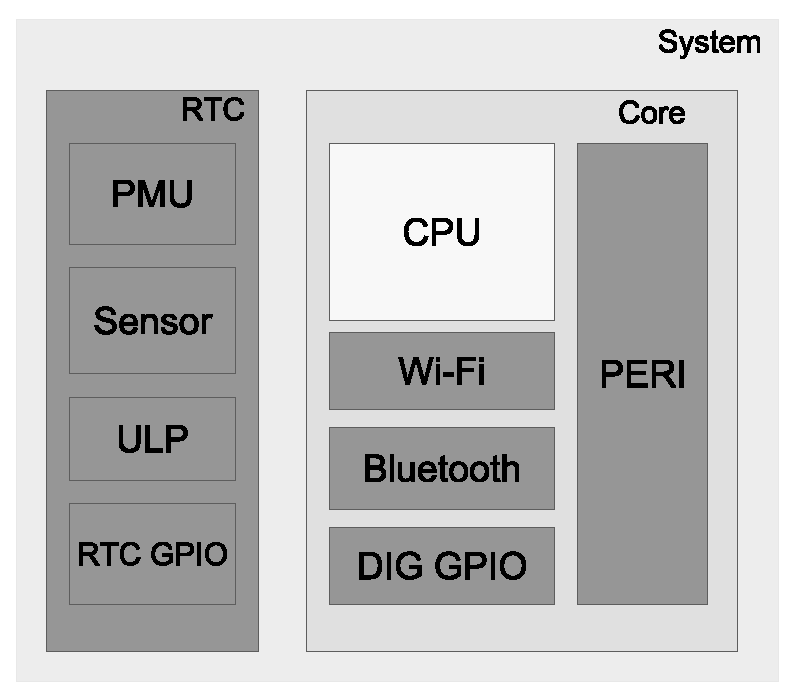
\includegraphics[width=0.5\textwidth]{./07-RESCLK/figures/reset_20211011.eps}
    \caption{系统复位}
    \label{figure:Reset}
\end{figure}

\begin{itemize}
    \item CPU复位：只复位 CPU 的所有寄存器。
    \item 内核复位：除了 RTC，会把整个 digital 的寄存器全部复位，包括 CPU、所有外设和数字 GPIO。
    \item 系统复位：会复位整个芯片所有的寄存器，包括 RTC。
\end{itemize}

\subsection{复位源}
大多数情况下，APP\_CPU 和 PRO\_CPU 将被立刻复位，有些复位源只能复位其中一个。APP\_CPU 和 PRO\_CPU 的复位原因也各自不同：当系统复位起来之后，PRO\_CPU可以通过读取寄存器 RTC\_CNTL\_RESET\_CAUSE\_PROCPU 来获取复位源，APP\_CPU 则可以通过读取寄存器 RTC\_CNTL\_RESET\_CAUSE\_APPCPU 来获取复位源。

表 \ref{table:resetreasons} 列出了从这些寄存器中可能读出的复位源。

\begin{longtable}[c]{ |l|l|l|l|m{8cm}| }
\caption{PRO\_CPU 和 APP\_CPU 复位源}
    \label{table:resetreasons}  \\
        \hline
        \rowcolor{lightgray}
        PRO & APP & 源 & 复位方式 & 注释\\
        \hline
        \endfirsthead
        \hline
       \rowcolor{lightgray}
        PRO & APP &  源 & 复位方式 & 注释 \\
        \hline
        \endhead
        \endfoot
        0x01 & 0x01 & 芯片上电复位 & 系统复位 &  - \\
        \hline
        0x10 & 0x10 & RWDT 系统复位 & 系统复位 & 详见 \hyperref[mod:wdt]{WDT 章节} \\
        \hline
        0x0F & 0x0F & 欠压复位 & 系统复位 & 详见 Power Management 章节\\
        \hline
        0x03 & 0x03 & 软件系统复位 & 内核复位 & 配置 \hyperref[fielddesc:RTCCNTLSWSYSRST]{RTC\_CNTL\_SW\_SYS\_RST} 寄存器\\
        \hline
        0x05 & 0x05 & Deep Sleep Reset & 内核复位 & 详见 Power Management 章节 \\
        \hline
        0x06 & 0x06 & SDIO Reset & 内核复位 & 保留
        \\\hline
        0x07 & 0x07 & MWDT0 全局复位 & 内核复位 & 详见 \hyperref[mod:wdt]{WDT 章节} \\
        \hline
        0x08 & 0x08 & MWDT1 全局复位 & 内核复位 & 详见 \hyperref[mod:wdt]{WDT 章节} \\
        \hline
        0x09 & 0x09 & RWDT 内核复位 & 内核复位 & 详见 \hyperref[mod:wdt]{WDT 章节} \\
        \hline
        0x0B & - & MWDT0 CPU 复位 & CPU 复位 & 详见 \hyperref[mod:wdt]{WDT 章节}  \\
        \hline
        0x0C & - & 软件 CPU 复位 & CPU 复位 &  配置 \hyperref[fielddesc:RTCCNTLSWAPPCPURST]{RTC\_CNTL\_SW\_APPCPU\_RST} 寄存器\\
		\hline
        - & 0x0B & MWDT1 CPU 复位 & CPU 复位 & 详见 \hyperref[mod:wdt]{WDT 章节} \\
        \hline
        - & 0x0C & 软件 CPU 复位 & CPU 复位 &  配置 \hyperref[fielddesc:RTCCNTLSWAPPCPURST]{RTC\_CNTL\_SW\_APPCPU\_RST} 寄存器\\
        \hline
        0x0D & 0x0D & RWDT CPU 复位 & CPU复位 & 详见 \hyperref[mod:wdt]{WDT章节}\\
        \hline
         - &  0xE &  PRO CPU 复位 &  CPU 复位 & 表明 PRO CPU 能够通过配置 \hyperref[DPORTAPPCPURESETTING]{DPORT\_APPCPU\_RESETTING} 寄存器单独复位 APP CPU \\
        \hline
    \end{longtable}

\section{系统时钟}


\subsection{概述}

ESP32提供了多种不同频率的时钟选择，可以灵活的配置CPU，外设，以及RTC的工作频率 ，以满足不同功耗和性能需求。下图 \ref{figure:Clock} 为系统时钟结构。

\begin{figure}[H]
    \centering
    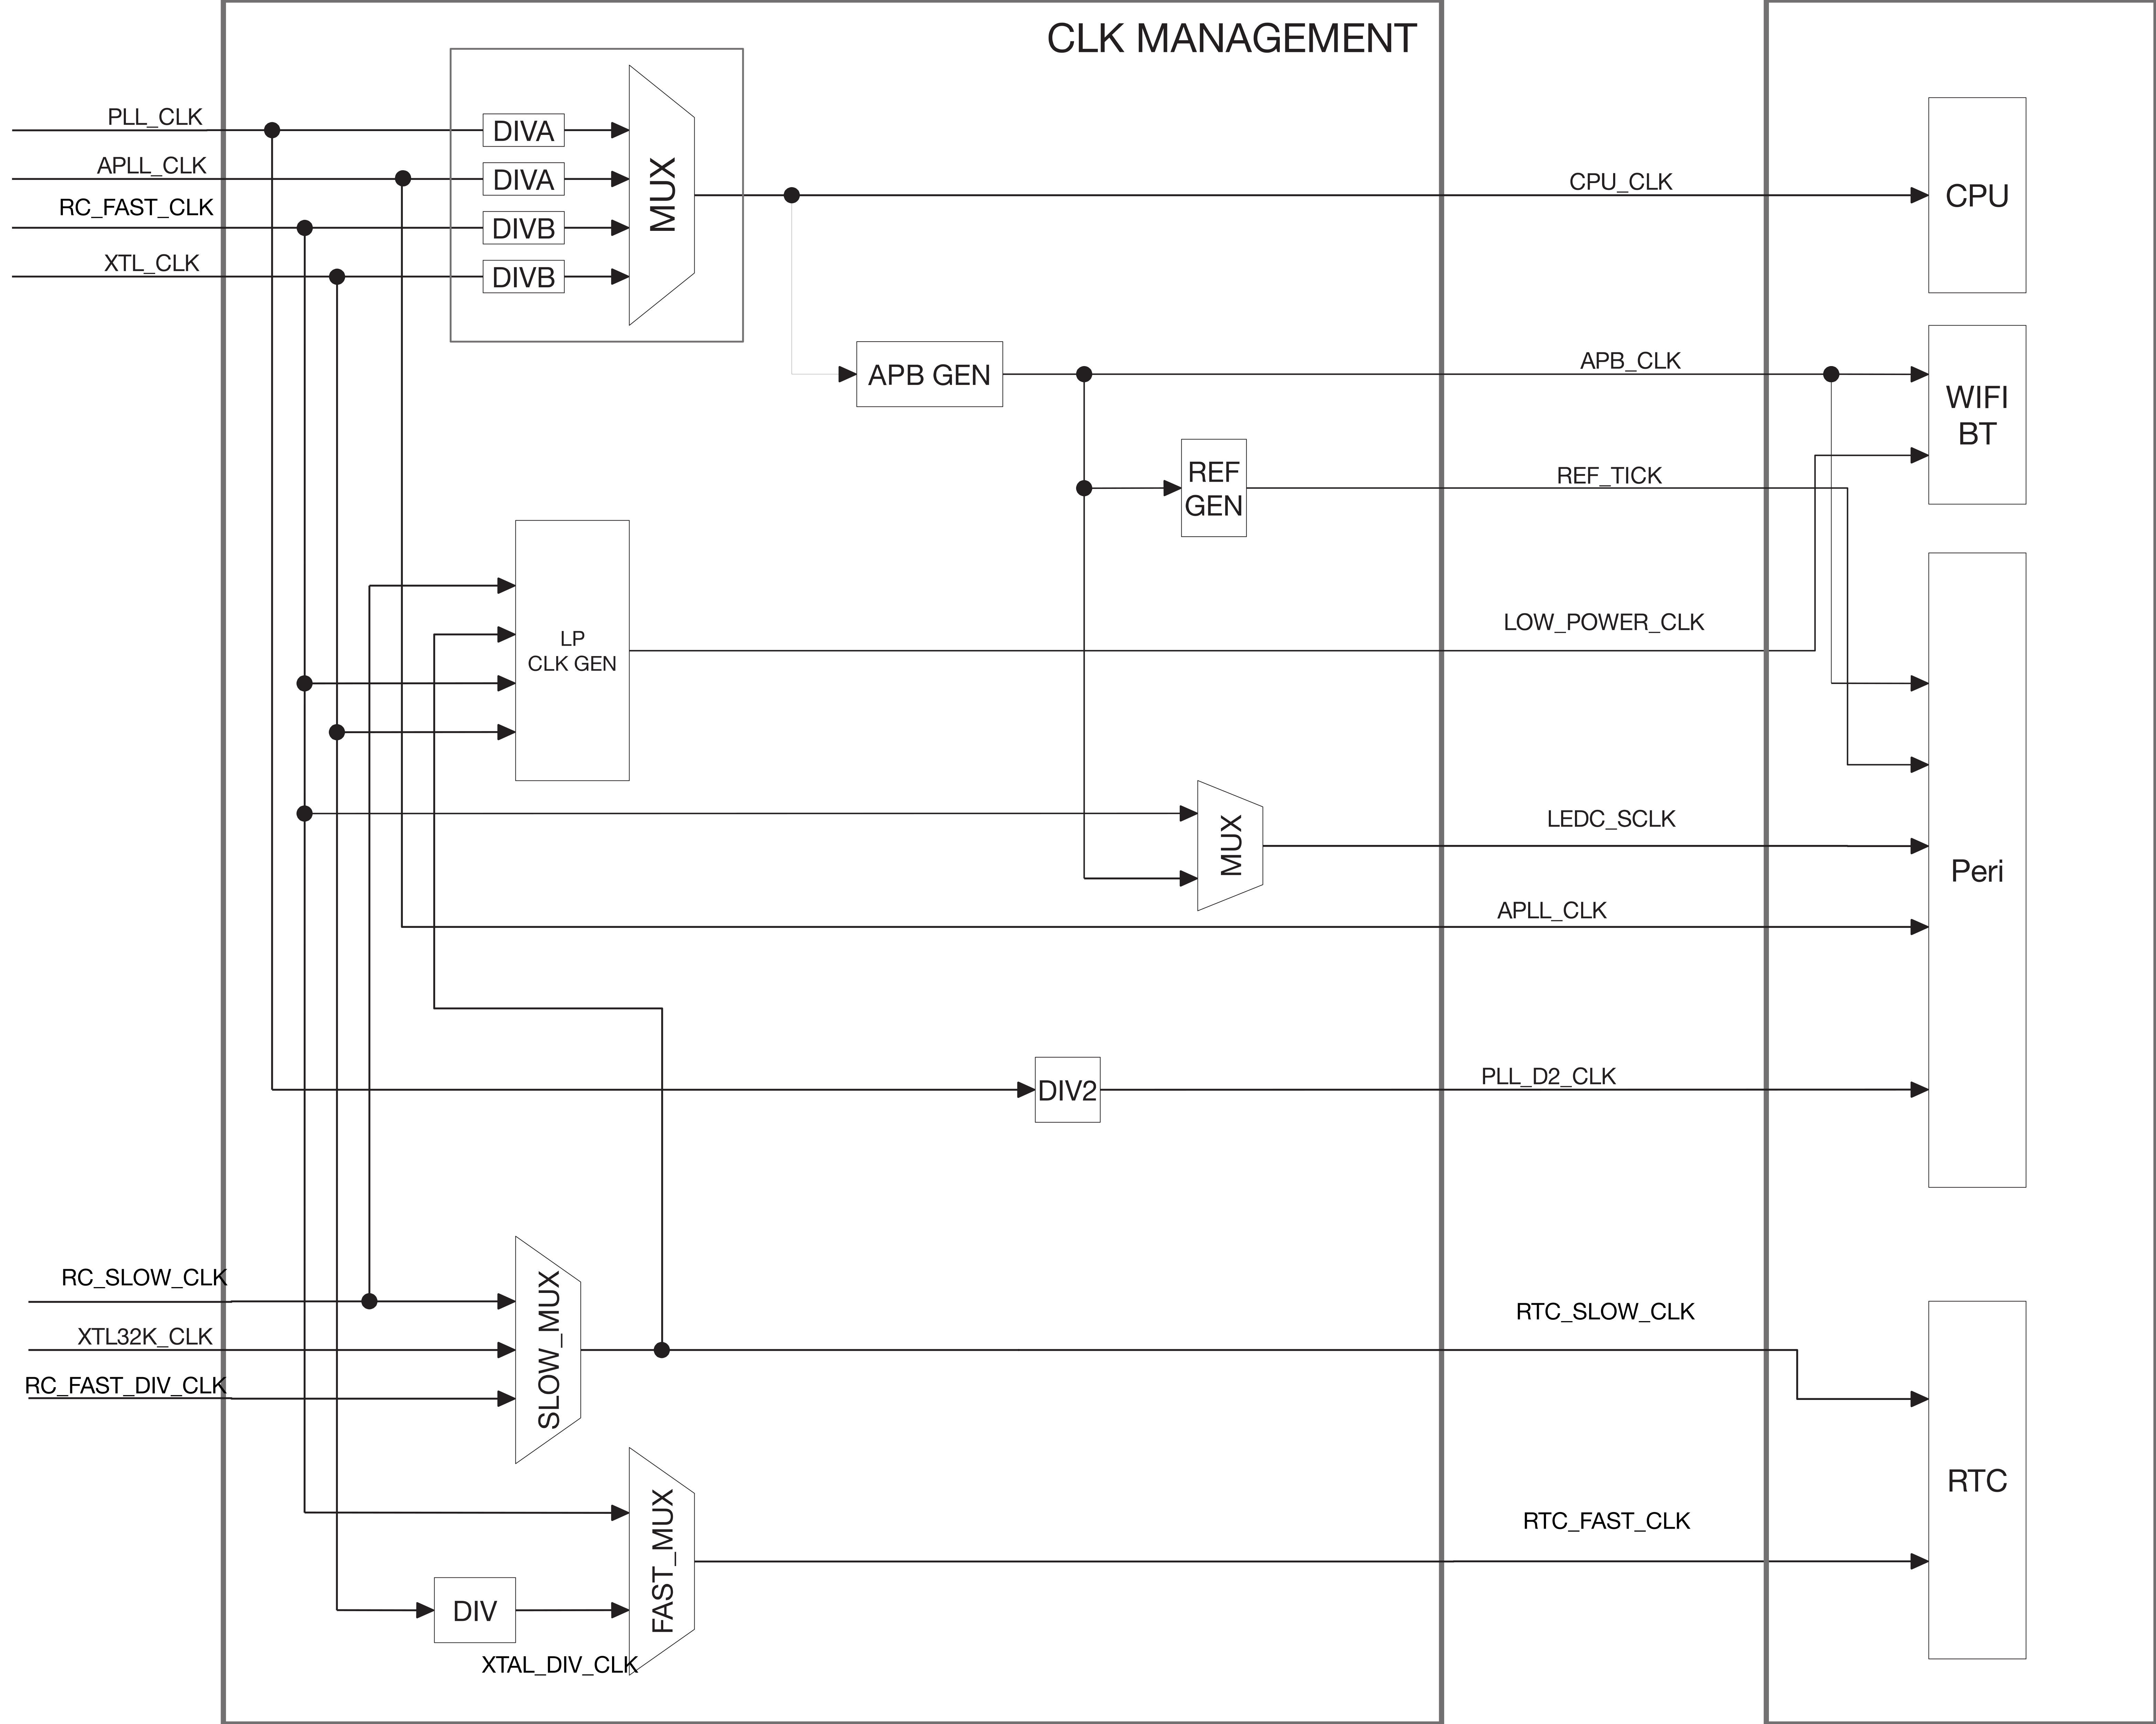
\includegraphics[width=1.0\textwidth]{./07-RESCLK/figures/clock.png}
    \caption{系统时钟}
    \label{figure:Clock}
\end{figure}

\subsection{时钟源}
ESP32 的时钟源分别来自外部晶振、内部 PLL 或振荡电路。具体地说，这些时钟源为：
\begin{itemize}
    \item 快速时钟
        \begin{itemize}
            \item PLL\_CLK，320 MHz 或 480 MHz 内部 PLL 时钟
            \item XTL\_CLK，2 \verb+~+ 40 MHz 外部晶振时钟
        \end{itemize}
    \item 低功耗慢速时钟
        \begin{itemize}
            \item XTL32K\_CLK，32 KHz 外部晶振时钟
            \item RC\_FAST\_CLK ，8 MHz 内部时钟，频率可调
	        \item RC\_FAST\_DIV\_CLK 由 RC\_FAST\_CLK 经 256 分频所得，频率为 (RC\_FAST\_CLK/256)。当 RC\_FAST\_CLK 的初始频率为 8 MHz 时，该时钟以 31.250 KHz 的频率运行。
	        \item RC\_SLOW\_CLK，150 KHz 内部低功耗时钟，频率可调
	    \end{itemize}
    \item 音频时钟
        \begin{itemize}
            \item APLL\_CLK，16 \verb+~+ 128 MHz 内部 Audio PLL 时钟
	    \end{itemize}
\end{itemize}

\subsection{CPU 时钟}

如图 \ref{figure:Clock} 所示，CPU\_CLK 为 CPU 主时钟，它在高效工作模式下，主频可以达到 240 MHz。同时，CPU 能够在超低频下工作，以减少功耗。

CPU\_CLK 由 \hyperref[regdesc:RTCCNTLSOCCLKSEL]{RTC\_CNTL\_SOC\_CLK\_SEL} 来选择时钟源，允许选择 PLL\_CLK，APLL\_CLK，RC\_FAST\_CLK，XTL\_CLK 作为 CPU\_CLK 的时钟源。具体请参考表 \ref{table:cpu clksrc} 和表 \ref{table:cpu clk}。
\begin{longtable}[c]{|l|l| }
       \caption{CPU\_CLK 源}
		\label{table:cpu clksrc}
	    \\\hline
        \rowcolor{lightgray}
       \hyperref[regdesc:RTCCNTLSOCCLKSEL]{RTC\_CNTL\_SOC\_CLK\_SEL} 值 & 时钟源 \\
        \hline
        0 & XTL\_CLK \\
        \hline
        1 & PLL\_CLK \\
        \hline
        2 & RC\_FAST\_CLK \\
        \hline
        3 & APLL\_CLK \\
        \hline
\end{longtable}


\begin{longtable}[c]{|l|l|l|m{10cm}|}
	\caption{CPU\_CLK 源}
    \label{table:cpu clk}
        \\\hline
        \rowcolor{lightgray}
        时钟源 & *SEL\_0 & *SEL\_1 & CPU 时钟 \\
        \hline
		XTL\_CLK & 0 & - & CPU\_CLK = XTL\_CLK / (\hyperref[fielddesc:SYSCONPREDIVCNT]{SYSCON\_PRE\_DIV\_CNT}+1)\\
        \hline
      PLL\_CLK (320 MHz) & 1  & 0 & CPU\_CLK = PLL\_CLK / 4 \newline
         		CPU\_CLK 频率为 80 MHz \\
        \hline
       PLL\_CLK (320 MHz) & 1  & 1  & CPU\_CLK = PLL\_CLK / 2 \newline
       			CPU\_CLK 频率为 160 MHz \\
        \hline
        PLL\_CLK (480 MHz) & 1 & 2 & CPU\_CLK = PLL\_CLK / 2 \newline
       			CPU\_CLK 频率为 240 MHz
       			\\\hline
       RC\_FAST\_CLK & 2  &  - & CPU\_CLK = RC\_FAST\_CLK / (\hyperref[fielddesc:SYSCONPREDIVCNT]{SYSCON\_PRE\_DIV\_CNT}+1)\\
        \hline
        APLL\_CLK & 3 & 0 & CPU\_CLK = APLL\_CLK / 4 \\
        \hline
        APLL\_CLK & 3 & 1 & CPU\_CLK = APLL\_CLK / 2 \\
        \hline
    \end{longtable}
    \vspace{-1em}
*SEL\_0：寄存器 \hyperref[regdesc:RTCCNTLSOCCLKSEL]{RTC\_CNTL\_SOC\_CLK\_SEL} 的值  \\
*SEL\_1：寄存器 \hyperref[fielddesc:CPUCPUPERIODSEL]{CPU\_CPUPERIOD\_SEL} 的值

\subsection{外设时钟}
外设所需要的时钟包括APB\_CLK，REF\_TICK，LEDC\_SCLK，APLL\_CLK 和 PLL\_F160M\_CLK。\\
下表 \ref{table:peri clk owner} 为接入各个外设的时钟。

\begin{longtable}[c]{ |l|l|l|l|l|l| }
 \caption{外设时钟用法}
    \label{table:peri clk owner}
        \\\hline
        \rowcolor{lightgray}
        外设 & APB\_CLK & REF\_TICK & LEDC\_SCLK & APLL\_CLK & PLL\_F160M\_CLK\\
        \hline
        EMAC & Y & N & N & Y & N \\
        \hline
        TIMG & Y & N & N & N & N \\
        \hline
        I2S & Y & N & N & Y & Y \\
        \hline
        UART & Y & Y & N & N & N \\
        \hline
        RMT & Y & Y & N & N & N \\
        \hline
        LED PWM & Y & Y & Y & N & N \\
        \hline
        PWM & Y & N & N & N & Y \\
        \hline
        I2C & Y & N & N & N & N \\
        \hline
        SPI & Y & N & N & N & N \\
        \hline
        PCNT & Y & N & N & N & N \\
        \hline
        eFuse Controller & Y & N & N & N & N \\
        \hline
        SDIO Slave & Y & N & N & N & N \\
        \hline
        SDMMC & Y & N & N & N & N \\
        \hline
    \end{longtable}

\vspace{-2em}
\subsubsection{APB\_CLK}

APB\_CLK 时钟频率由 CPU\_CLK 源决定，具体见表 \ref{table:apb_clk_src}：

\begin{longtable}[c]{|l|l|}
      \caption{APB\_CLK}
    \label{table:apb_clk_src}
        \\\hline
        \rowcolor{lightgray}
        CPU\_CLK 源 & APB\_CLK 时钟频率\\
        \hline
        \endfirsthead
        \hline
        \rowcolor{lightgray}
        CPU\_CLK 源 & APB\_CLK \\
        \hline
        \endhead
        \endfoot
        PLL\_CLK & 80 MHz \\
        \hline
        APLL\_CLK & CPU\_CLK / 2 \\
        \hline
        XTL\_CLK & CPU\_CLK \\
        \hline
        RC\_FAST\_CLK & CPU\_CLK \\
        \hline
\end{longtable}

\subsubsection{REF\_TICK}\label{sec:ref_tick}

REF\_TICK 时钟频率由 APB\_CLK 分频产生，APB\_CLK 时钟频率由 CPU\_CLK 源决定。REF\_TICK 的时钟频率应固定，因此当切换 CPU\_CLK 源时，应配置分频寄存器，使其频率固定。分频寄存器如何配置见表 \ref{table:ref_tick}：

\begin{longtable}[c]{|l|l|l|}
      \caption{REF\_TICK}
    \label{table:ref_tick}
        \\\hline
        \rowcolor{lightgray}
        CPU\_CLK 源 & APB\_CLK 时钟频率 & REF\_TICK 频率\\
        \hline
        \endfirsthead
        \hline
        \rowcolor{lightgray}
        CPU\_CLK 源 & APB\_CLK 时钟频率 & REF\_TICK 频率\\
        \hline
        \endhead
        \endfoot
        PLL\_CLK & 80 MHz & APB\_CLK / (\hyperref[fielddesc:SYSCONPLLTICKNUM]{SYSCON\_PLL\_TICK\_NUM}+1)\\
        \hline
        APLL\_CLK & CPU\_CLK / 2 & APB\_CLK / (\hyperref[fielddesc:SYSCONAPLLTICKNUM]{SYSCON\_APLL\_TICK\_NUM}+1)\\
        \hline
        XTL\_CLK & CPU\_CLK & APB\_CLK / (\hyperref[fielddesc:SYSCONXTALTICKNUM]{SYSCON\_XTAL\_TICK\_NUM}+1)\\
        \hline
        RC\_FAST\_CLK & CPU\_CLK & APB\_CLK / (\hyperref[fielddesc:SYSCONCK8MTICKNUM]{SYSCON\_CK8M\_TICK\_NUM}+1)\\
        \hline
\end{longtable}

例如，当 REF\_TICK 时钟频率固定为 1 MHz 时，如果 CPU\_CLK 源为 PLL\_CLK，则 REF\_TICK 频率 = 80 MHz / (SYSCON\_PLL\_TICK\_NUM+1) = 1 MHz，那么 SYSCON\_PLL\_TICK\_NUM 应配置为 79 (0x4F)。


\subsubsection{LEDC\_SCLK 源}

LEDC\_SCLK 时钟源由寄存器 LEDC\_APB\_CLK\_SEL 决定，如表 \ref{table:led_sclk} 所示。

\begin{longtable}[c]{|l|l|} \caption{LEDC\_SCLK 源}
    \label{table:led_sclk}
        \\\hline
        \rowcolor{lightgray}
        LEDC\_APB\_CLK\_SEL 值 & LEDC\_SCLK 源  \\
        \hline
        0 & RC\_FAST\_CLK \\
        \hline
        1 & APB\_CLK \\
        \hline
\end{longtable}

\subsubsection{APLL\_SCLK 源}

APLL\_CLK来自内部PLL\_CLK，其输出频率通过使用 APLL 配置寄存器来配置。

\subsubsection{PLL\_F160M\_CLK 源}

PLL\_F160M\_CLK 是 PLL\_CLK 根据当前 PLL 的频率自动调节分频系数所得，频率时钟为 160 MHz。


\subsubsection{时钟源注意事项}

大多数外设一般在选择 PLL\_CLK 时钟源的情况下工作。若频率发生变化，外设需要通过修改配置才能以同样的频率工作。接入REF\_TICK的外设允许在切换时钟源的情况下，不修改外设配置即可工作。详情请参考表 \ref{table:peri clk owner}。

LED PWM 模块能将 RC\_FAST\_CLK 作为时钟源使用，即在 APB\_CLK 关闭的时候，LED PWM 也可工作。换而言之，当系统处于低功耗模式时（参考章节 \ref{mod:lowpowm} \textit{\nameref{mod:lowpowm}}），所有正常外设都将停止工作（APB\_CLK 关闭），但是 LED PWM 仍然可以通过 RC\_FAST\_CLK 来正常工作。



\subsection{Wi-Fi BT 时钟}
Wi-Fi 和 BT 必须在 APB\_CLK 时钟源选择 PLL\_CLK 下才能工作。只有当 Wi-Fi 和 BT 同时进入低功耗模式时，才能暂时关闭 PLL\_CLK。

LOW\_POWER\_CLK 允许选择 XTL32K\_CLK、\hyperlink{SLOW_CLK}{RTC\_SLOW\_CLK}、RC\_FAST\_CLK 或 XTL\_CLK，用于 Wi-Fi  和 BT 的低功耗模式。


\subsection{RTC 时钟}

RTC\_SLOW\_CLK 和 RTC\_FAST\_CLK 的时钟源为低频时钟。 RTC 模块能够在大多数时钟源关闭的状态下工作。


RTC\_SLOW\_CLK 允许选择 RC\_SLOW\_CLK，XTL32K\_CLK 或 RC\_FAST\_DIV\_CLK，用于驱动 Power Management 模块。

RTC\_FAST\_CLK 允许选择 XTL\_CLK 的分频时钟或 RC\_FAST\_CLK，用于驱动 On-chip Sensor 模块。

\subsection{音频 PLL}\label{audiopll}
音频应用和其他对于数据传输时效性要求很高的应用都需要高度可配置、低抖动并且精确的时钟源。来自系统时钟的时钟源可能会携带抖动，并且不支持高精度的时钟频率配置。


为了通过集成的精密时钟源来最大限度地降低系统成本，ESP32 集成了音频 PLL。Audio PLL 公式如下：

\[
f_{\rm{out}} = \frac{f_{\rm{xtal}}(\rm{sdm2}+\frac{\rm{sdm1}}{2^8}+\frac{\rm{sdm0}}{2^{16}}+4)}{2(odiv+2)}
\]

其中，
\begin{itemize}
    \item \begin{math}f_{\rm{xtal}}\end{math}：晶振频率，通常为 40 MHz
    \item sdm0：可配参数 0 \verb+~+ 255
    \item sdm1：可配参数 0 \verb+~+ 255
    \item sdm2：可配参数 0 \verb+~+ 63
    \item odiv：可配参数 0 \verb+~+ 31
    \item 公式的分子频率工作范围在350 MHz \verb+~+ 500 MHz

\[
350 MHz<{f_{\rm{xtal}}(\rm{sdm2}+\frac{\rm{sdm1}}{2^8}+\frac{\rm{sdm0}}{2^{16}}+4)}<500 MHz
\]

\end{itemize}

注意：sdm1 和 sdm0 在 ESP32 的 revision0 版本中不支持。更多关于 ESP32 版本的信息，可在 \href{\linkprefix\linkchiperrataCN}{\chipseries{} 系列芯片勘误表} 中查看。

Audio PLL 可通过寄存器RTC\_CNTL\_PLLA\_FORCE\_PU 强行打开，或者通过寄存器 RTC\_CNTL\_PLLA\_FORCE\_PD 强行关闭，关闭优先级大于打开优先级。当 RTC\_CNTL\_PLLA\_FORCE\_PU 和 RTC\_CNTL\_PLLA\_FORCE\_PD 同时为 0 的时候，PLL 会跟随系统状态，当系统进入睡眠模式的时候自动关闭，系统被唤醒的时候自动打开。

\section{寄存器列表}\label{sec:resclk-reg-summ}

本小节的所有地址均为相对于 SYSCON 基地址的地址偏移量（相对地址），具体基地址见章节 \ref{mod:sysmem} \textit{\nameref{mod:sysmem}} 中的表 \ref{table:Peripheral_Address_Mapping} \textit{外设地址映射}。

\subfile{\modulefiles/apb-ctrl-summary_cn}

\section{寄存器}\label{sec:resclk-reg-desc}

本小节的所有地址均为相对于 SYSCON 基地址的地址偏移量（相对地址），具体基地址见章节 \ref{mod:sysmem} \textit{\nameref{mod:sysmem}} 中的表 \ref{table:Peripheral_Address_Mapping} \textit{外设地址映射}。

\subfile{\modulefiles/apb-ctrl-reg_cn}
\end{document}